\documentclass[11pt]{article}
\usepackage[utf8]{inputenc}
\usepackage[margin=0.8in]{geometry}
\usepackage{amsfonts, amsmath}
\usepackage{tikz}
\usepackage[nobreak=false]{mdframed}
\usepackage{pgf}
\usepackage{enumitem}
\usepackage{mathtools}
\usepackage{bbm}
\usepackage{bm}
\usepackage{graphicx}
\usepackage{url}
\usepackage{enumitem}
\usepackage{amsthm,amssymb}
\usepackage{minted}
\setlength\parindent{0pt}
\newcommand{\solution}{\subsection*{Solution:}}
\DeclareMathOperator*{\argmax}{arg\!max}
\DeclareMathOperator*{\argmin}{arg\!min}

\begin{document}
\title{EE127 Homework 2}
\author{Vighnesh Iyer}
\date{\today}
\maketitle

\subsection*{Exercise 1 (PCA and low-rank compression)}

We are given a $n \times m$ matrix $X = [x_1,\ldots,x_m]$, with $x_i \in \mathbb{R}^{n}$, $i=1,\ldots,m$ the data points.  We assume that the data matrix is centered, in the sense that $x_1+\ldots+x_m = 0$. In lecture, it was asserted that there is equivalence between three problems:
\begin{itemize}
    \item[($P_1$)] Finding a line going through the origin that maximizes the variance of the points projected on the line.
    \item[($P_2$)] Finding a line going through the origin that minimizes the sum of squares of the distances from the points to their projections;
    \item[($P_3$)] Finding a rank-one approximation to the data matrix.
\end{itemize}
In this exercise, you are asked to show the equivalence between these three problems.
\begin{enumerate}
    \item Consider the problem of projecting a point $x$ on a line ${\cal L} = \{x_0 + v u \::\: v \in \mathbb{R}\}$, with $x_0, \in \mathbb{R}^n$, $u^Tu=1$, given. Show that the projected point $z$ is given by $z = x_0+v^* u$, with $v^* = (x-x_0)^Tu$, and that the minimal squared distance $\|z-x\|_2^2$ is equal to $\|x-x_0\|_2^2 - ((x-x_0)^Tu)^2$.
    \item Show that problems $P_1,P_2$ are equivalent.
    \item Show that $P_3$ is equivalent to $P_1$. \emph{Hint: } show that the data matrix is rank-one if and only if the points are all on a line that goes through the origin.
\end{enumerate}

\begin{solution}
\begin{enumerate}
    \item From the livebook: "The \emph{projection} of a given point $x$ on the line ${\cal L}$ is a vector $v$ located on the line, that is closest to $x$ in (L2 norm)"
    \begin{align*}
        v^* &= \argmin_{v} \|x - x_0 - vu\|_2 \\
        &= \argmin_{v} \|(x - x_0) - vu\|_2^2 \\
        \text{Aside: } \|a-b\|_2^2 = \langle a-b,a-b \rangle &= \langle a,b \rangle + \langle a,-b \rangle + \langle -b,a \rangle + \langle -b,-b \rangle \\
        &= \|a\|_2^2 - 2 \langle a,b \rangle + \|b\|_2^2 = \|a\|_2^2 - 2a^Tb + \|b\|_2^2 \\
        v^* &= \argmin_v \|x-x_0\|_2^2 - 2(x-x_0)^T vu + \|vu\|_2^2 \\
        &= \argmin_v v^2 - 2vu^T (x-x_0) + C \text{ where } C \text{ is some constant } \\
        &= \argmin_v (v - u^T(x-x_0))^2 + C\\
        \rightarrow v^* &= u^T(x-x_0)
    \end{align*}

    The projected point $z$ is just going $v^*$ scalar distance on the line $\cal L$.
    \begin{align*}
        z = {\cal L} (v^*) = x_0 + v^* u
    \end{align*}

    We can directly calculate $\|z-x\|_2^2$:
    \begin{align*}
        \|z - x\|_2^2 &= \|x_0 + u^T(x-x_0)u -x\|^2_2 \\
        &= \|u^T(x-x_0)u - (x-x_0)\|_2^2 \\
        &= \|u^T(x-x_0)u\|_2^2 - 2(u^T(x-x_0)u)^T(x-x_0) + \|x-x_0\|^2 \\
        &= ((x-x_0)u^T)^2 - 2\|u^T(x-x_0)u\|^2_2 + \|x-x_0\|_2^2 \\
        &= -((x-x_0)u^T)^2 + \|x-x_0\|_2^2
    \end{align*}

\item For a line ${\cal L} = vu : v \in \mathbb{R}, u^Tu = 1, u \in \mathbb{R}^n$ passing through the origin with $m$ data points $x_1, \dots, x_m$, we can write both $P_1$ and $P_2$'s optimization problems.
    \begin{align*}
        P_1&: \argmax_u \sum_{i=1}^m (u^T x_i - u^T \hat{x})^2 \text{ where } \hat{x} = \frac{1}{m} (x_1 + \dots + x_m) \\
        &= \argmax_u \sum_{i=1}^m (u^T x_i)^2 \text{ due to } \hat{x} \text{ being constant} \\
        &= \argmax_u \sum_{i=1}^m \langle x_i, u \rangle^2 \\
        P_2&: \argmin_u \sum_{i=1}^m (x_i - u^T x_i u)^2 \\
        &= \argmin_u \sum_{i=1}^m dist(x_i, \langle x_i,u \rangle \cdot u)^2
    \end{align*}

    We can relate the relationship between the norm of $x_i$, the projection of $x_i$ onto line $\cal L$, and the distance between the projected point and the original $x_i$ using the Pythagorean thm:
    \begin{align*}
        dist(x_i, \langle x_i,u \rangle \cdot u)^2 + \langle x_i,u \rangle^2 = \|x_i\|_2^2
    \end{align*}
        Since the RHS of this expression is constant for each $x_i$, we can see that mimimizing the distance will lead to the same solution as maximizing the variance. This also applies to dimensions higher than $\mathbb{R}^2$.

\item
\begin{align*}
    P_1&: \argmax_u \sum_{i=1}^m \langle x_i,u \rangle^2 \\
    P_3&: \min_{A_1 \in \mathbb{R}^{nxm}} \|A - A_1\|_F^2 : rank(A_1) = 1
\end{align*}

If the points of $A$ all lie on a line ${\cal L} = vu$ then $\rangle x_i,u \langle = \|x_i\|_2$ for all $i$ because each point's projection on $\cal L$ is the point's distance from the origin. This also means $P_2$'s minimization expression will be zero.

We know that the solution to $P_3$ is the SVD decomposition with the largest singular value $A_1 = \sigma_1 u_1 v_1^T$. If $A$ is rank 1, then all other singular values will be zero, and $A_1$ perfectly reconstructs $A$.

If $P_2$ is reformulated as:
\begin{align*}
    P_2&: \argmin_{u,v,\sigma} (A - A_1)^2
\end{align*}

the minimum is zero only if $A_1$ perfectly reconstructs $A$ which implies that $P_3$ is equivalent to $P_2$. $P_2$ is already shown to be equivalent to $P_1$.
\end{enumerate}
\end{solution}

\newpage
\subsection*{Exercise 2 (Generalized Eigenvalues and Image Segmentation)}

In this exercise, we will implement an algorithm for image segmentation from a graph-theoretic approach. As a simplified problem, we will focus on separating the foreground of an image from its background. We provide you with a skeleton code in the archive image\_segmentation.zip that imports an image and guide you through the implementation.

An image is described as a matrix $M$ of shape (N, M) whose values represent the gray scale color normalized between zero and one. Even though we restrict now to gray images, please note that the same algorithm could be easily extended to colored images.

An undirected graph is a triplet $(V, E, W)$ where $V$ is the set of nodes, $E$ the set of edges, and $W$ the set of weights for each edge. As a first step, we would like to construct a graph that represents the image. For that purpose, we choose $V$ to be the set of pixels. We say that there is an edge $(i, j)$ between pixel $i$ and pixel $j$, $1 \leq i, j \leq NM$, if they are neighbors in the image ($\|X(i) - X(j) \|_2 \leq r$). For each edge $(i, j)$, we will use as weight $w_{ij} = e^{-\frac{|M[x_i][y_i] - M[x_j][y_j]|}{\sigma_i}} * e^{\frac{-\sqrt{(x_i - x_j)^2 + (y_i - y_j)^2}}{\sigma_x}}$, where $(x_i, y_i)$ represents the location of pixel $i$ and $(x_j, y_j)$ represents the location of pixel $j$. This is a measure of pixel similarity. Finally, we are interested in the whole affinity matrix $W$ of shape $(NM, NM)$, where each entry has the value zero is there is no edge between the pixels and the value $w_{ij}$ if there is an edge.

\begin{enumerate}
    \item Complete the code in the notebook \texttt{image-seg.ipynb} that transforms the image \texttt{img-cup-small.png} into the affinity matrix $W$. The tuned parameters $\sigma_x, \sigma_i, r$ are provided in the notebook.
\end{enumerate}

% Let $W$ be the affinity matrix of the graph.
Let $D$ be the diagonal matrix of shape $(NM, NM)$, where the $i^{th}$ entry equals the sum of weights associated with edges incident on pixel $i$. That is, $D(i) = \sum_{j} W(i, j)$. We wish to solve the generalized eigenvalue problem $(D - W)y = \lambda Dy$ for all eigenvectors and all eigenvalues.

This eigenvalue problem is a known approximation to finding a partition of a graph that minimize the normalized cut in graph theory. Also, if the graph is connected, then the largest eigenvalue of the adjacency matrix as well as the smallest eigenvalue of the Laplacian have multiplicity 1. We can expect that the gap between this and the nearest eigenvalue is related to some kind of connectivity measure of the graph (for more information on the general topic of graph eigenvalues, one can refer to \url{http://web.cs.elte.hu/~lovasz/eigenvals-x.pdf}). The partition that approximate the solution to the normalized cut problem is derived from the generalized eigenvector with the second smallest eigenvalue and can be straightforwardly used in image segmentation.

\begin{enumerate}
    \item[2.] Explain how to relate this problem to the symmetric eigenvalue problem we saw in class. Furthermore, explain how you would solve this problem provided routine code to compute a SVD.
\end{enumerate}

\begin{enumerate}
    \item[3.] Find the generalized eigenvector $y$ for the eigenvector with the second smallest eigenvalue in the case of your given image. You will rely on linear algebra routine libraries like \texttt{numpy.linalg}.
\end{enumerate}

The $i$-th entry of y can be viewed as a “soft” indicator of the component membership of the $i$-th pixel.

\begin{enumerate}

\item[4.] Use this indication to transform your image into a binary image (the so-called result of image segmentation). Try separating pixels corresponding to positive / negative values and above the median / below the median values of the entries of $y$ to split the image into two components. Plot the obtained binary image and the second eigenvector's heatmap. How might we improve our image segmentation results to obtain a segmentation that resembles our heatmap, but with sharper segmentations? Hint: consider a recursive approach to graph partitioning.
\end{enumerate}

\begin{solution}
\begin{enumerate}
\item I used the following code to compute the affinity matrix $W$ and the diagonal matrix $D$. It is very inefficient.
    \begin{minted}[tabsize=2,breaklines]{python}
W = np.zeros((M.shape[0] * M.shape[1], M.shape[0] * M.shape[1]))
for i in range(M.shape[0]*M.shape[1]):
    for j in range(M.shape[0]*M.shape[1]):
        pixel_i = (int(i / M.shape[1]), int(i % M.shape[1]))
        pixel_j = (int(j / M.shape[1]), int(j % M.shape[1]))
        if (np.sqrt((pixel_i[0] - pixel_j[0])**2 + (pixel_i[1] - pixel_j[1])**2) <= r):
            W[i,j] = np.exp(-abs(M[pixel_i[0],pixel_i[1]] - M[pixel_j[0],pixel_j[1]]) / sigma_i) * \
                np.exp(-np.sqrt((pixel_i[0] - pixel_j[0])**2 + (pixel_i[1] - pixel_j[1])**2) / sigma_x)
        else:
            W[i,j] = 0
D = np.sum(W, axis=1)
\end{minted}

\item The symmetric eigenvalue problem refers to applying the spectral theorem applied to a symmetric matrix $A$.
\begin{align*}
    A = U \Lambda U^T
\end{align*}
where $U$ is a matrix constructed using the eigenvectors of $A$ as columns, and $\Lambda$ is a diagonal matrix with $A$'s eigenvalues.

The problem $(D-W)y = \lambda D y$ is similar to the symmetric eigenvalue problem since $D-W$ is a symmetric matrix and we want to obtain the eigenvalues of that matrix to find $y$ and $\lambda$. But we have to account for the RHS having the additional factor of $D$. We can correct this:

\begin{itemize}
    \item First find the eigenvalues $\lambda_i$ and respective eigenvectors $y_{Ai}$ for $D-W$ using SVD
    \item Then find the original eigenvectors as $y_i = \text{element-wise divide}(y_{Ai}, diag(D))$
\end{itemize}

\item
\begin{minted}{python}
w,v = np.linalg.eig(np.diag(D)-W)
order = np.argsort(np.abs(w)) # ascending order
eigv_2 = np.divide(v[:,order[1]], D)
\end{minted}

\item
\begin{figure}[H]
    \centerline{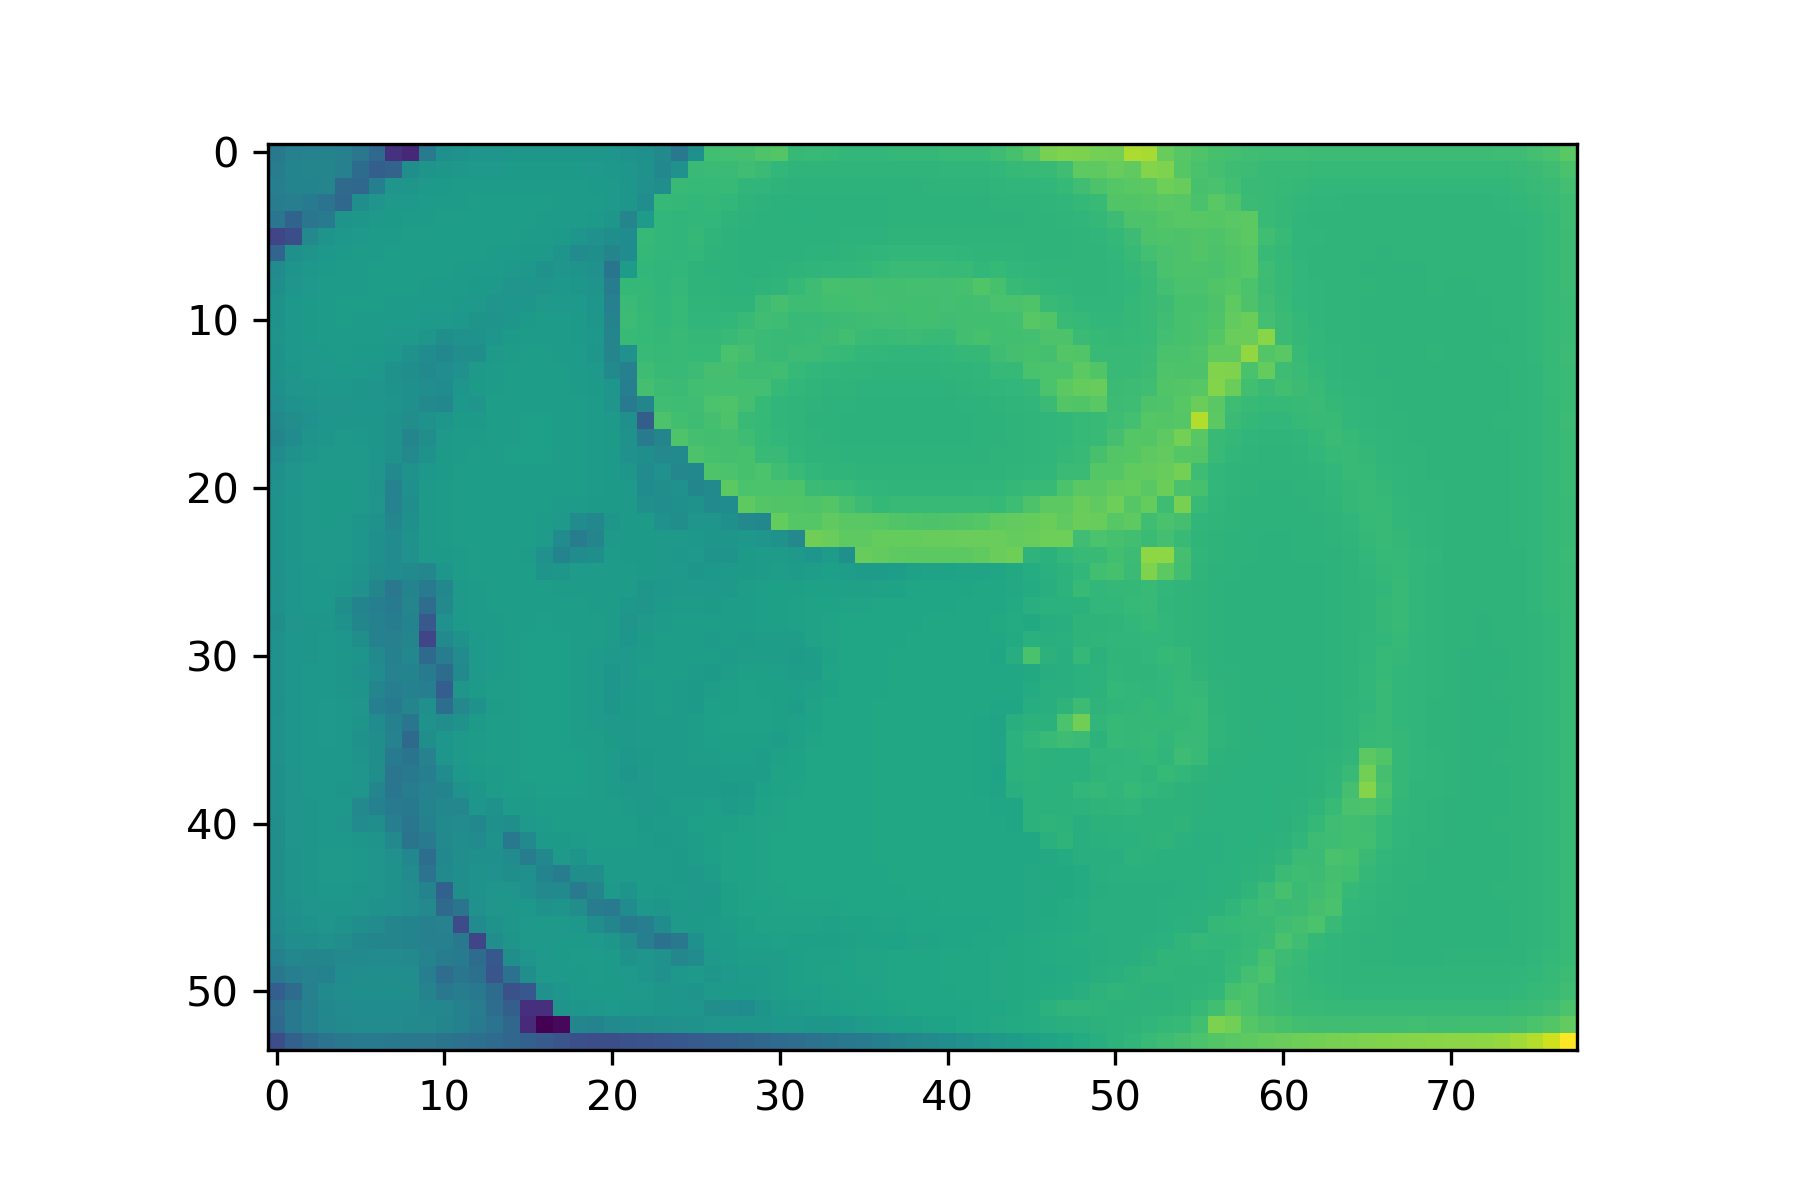
\includegraphics[width=0.5\textwidth]{figs/heatmap_eig2.png}}
\end{figure}

\begin{figure}[H]
    \centerline{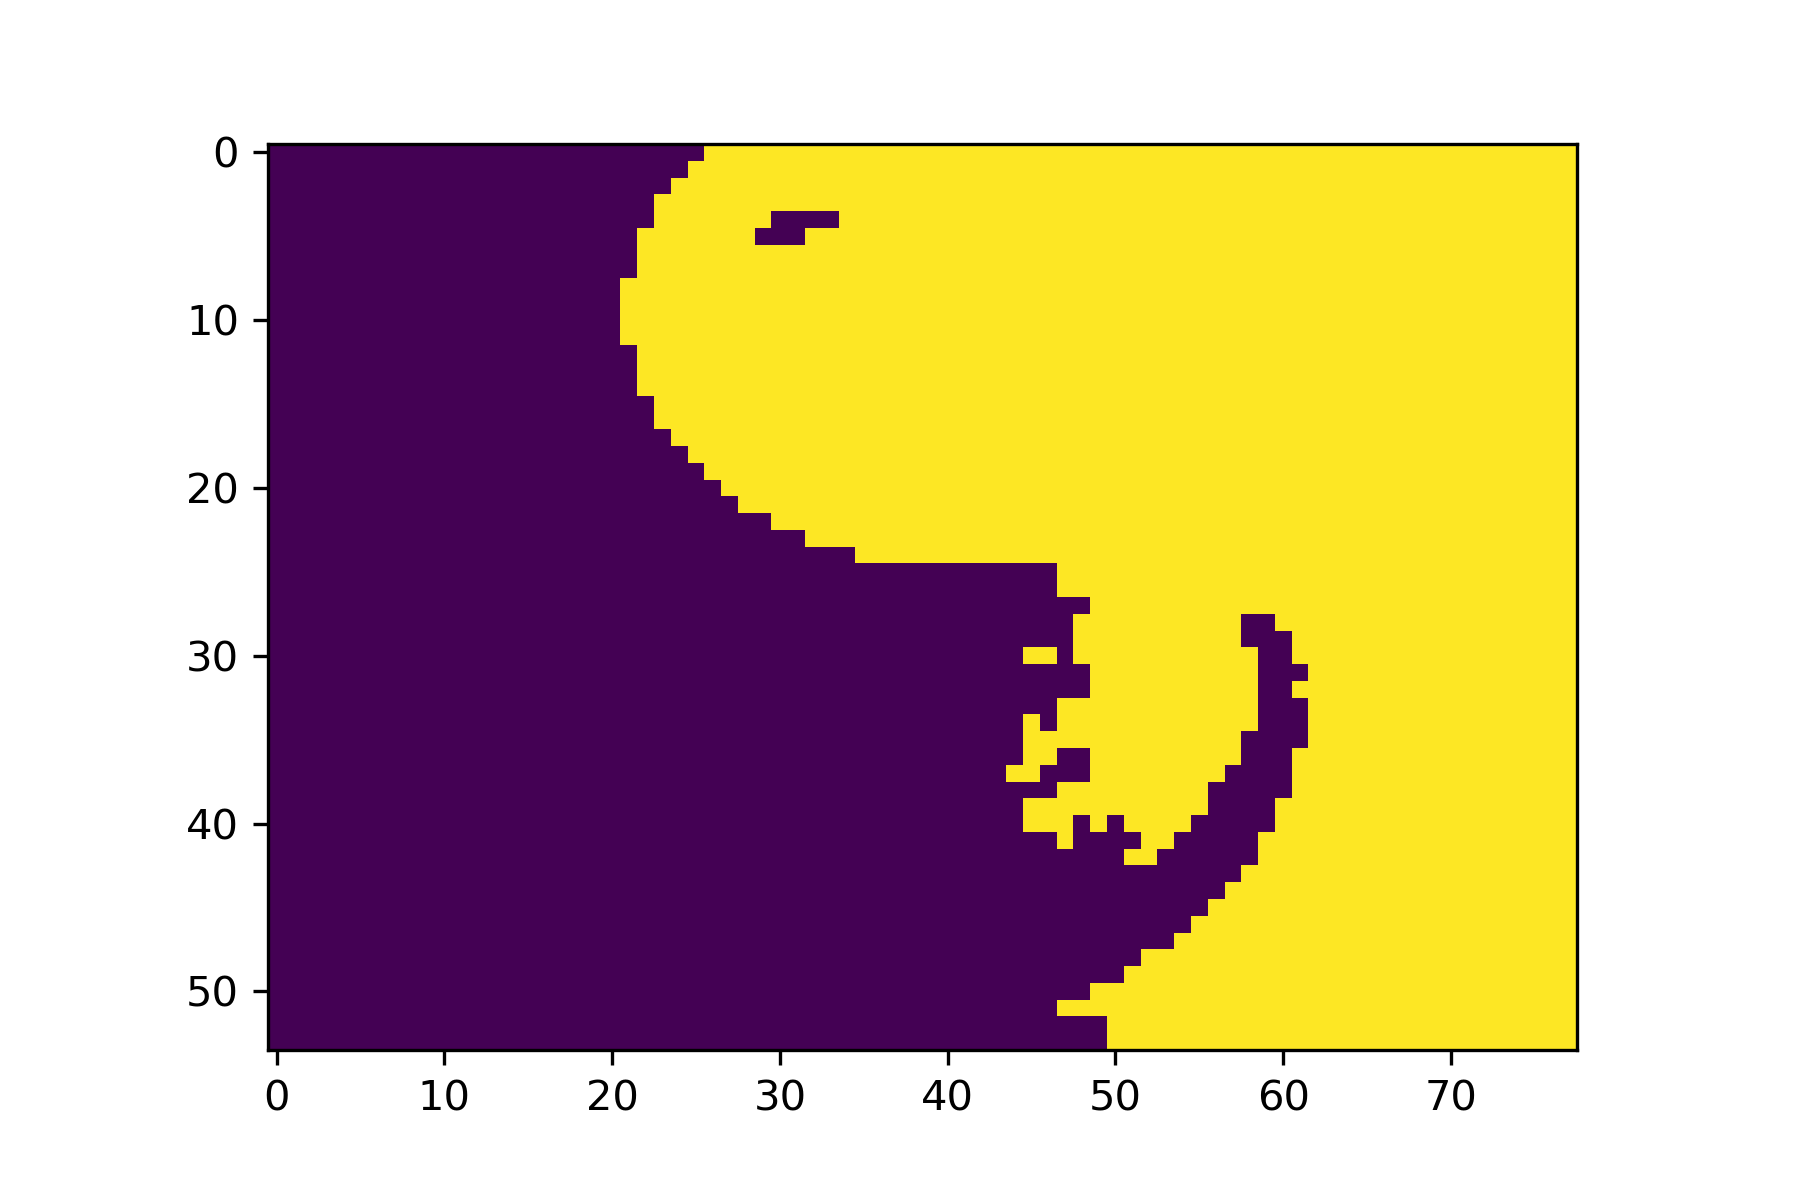
\includegraphics[width=0.5\textwidth]{figs/binary_eig2.png}}
\end{figure}

It looks like the partition was between the rim of the cup and its surroundings from the rest of the image for the second smallest eigenvalue. This algorithm can be improved by recursively applying it (construct W, find the most partition that miminizes the cut, 'de-weight' each edge that belongs to the partition selected by the 2nd smallest eigenvalue by taking $v_{-2}^T W$ and subtracting it from $W$, and rerun the partitioning by finding a new SVD).
\end{enumerate}
\end{solution}

\newpage
\subsection*{Exercise 3 (PCA and Senate Voting Data)}

We return to the Senate voting data examined in HW1, with $X$ the $m \times n$ data matrix, where each row corresponds to a Senator, and each column to a bill.
\begin{enumerate}
    \item Find a $n$-vector $a$ and scalar $b$ such that the variance of the corresponding score function $f(x) = a^Tx+b$ is maximized. (\textbf{Correction:} there is a condition that $a^T a = 1$)
    \item How does the variance obtained previously compare to the one obtained with $a$ set to the center of the data points, and $b$ set so that the average score is zero? Comment on the phrase ``senators vote according to the party average''.
    \item What is the total variance explained by the first two principal components? Plot the data projected on the corresponding plane.
    \item Based on the first principal component, which bill(s) would you say have been the most important? Which Senators are the most "extreme"?
\end{enumerate}

\begin{solution}
\begin{enumerate}
\item We let the 'score function' of each row vector be $f(x) = a^T x + b$, and can find the aggregate variance across all rows.
    \begin{align*}
        \text{Aggregate variance of } f(x) &= \sum_{i=1}^m (f(x_i) - \overline{f(x_i)})^2 \\
        &= \sum_{i=1}^m (a^T x_i + b - (a^T \hat{x} - b))^2 \text{ where } \hat{x} = \frac{1}{m}(x_i + \dots + x_m) \\
        &= \sum_{i=1}^m (a^T x_i - a^T \hat{x})^2
    \end{align*}
    So this reduces to the standard variance maximization problem, whose solution $a$ is the eigenvector with the largest eigenvalue for the covariance matrix of $X$. $b$ can be any scalar as it doesn't affect the variance of the scores.
\begin{minted}{python}
C = np.cov(X.T, bias=True)
w, v = np.linalg.eig(C)
a = v[:,0]
[np.var(X @ v[:,i]) for i in range(len(w))]
[149.74896507620727,
 25.422196529024113,
 12.243420297952678,
 6.490267033734414,
 6.063968727871187,
 5.563914277806253,
 4.798536085393635,
    ...
\end{minted}

\item
\begin{minted}{python}
a_new = np.mean(X, axis=0)
a_new = a_new / np.linalg.norm(a_new)
b_new = np.mean(X @ a_new)
np.var(X @ a_new - b_new)
13.414789689563143
\end{minted}
So the variance with this combo of $a$ and $b$ is much smaller than the ideal $a$.
There seems to be a pattern of senators voting (mostly in favor of a bill) as an entire bloc.
\begin{minted}{python}
reds = [i for i, x in enumerate(affiliations) if x == 'Red']
blues = [i for i, x in enumerate(affiliations) if x == 'Blue']
red_means = np.mean(X[reds,:],axis=0) / np.linalg.norm(X[reds,:],axis=0)
blue_means = np.mean(X[blues,:],axis=0) / np.linalg.norm(X[blues,:],axis=0)

print(np.mean(X[reds,:] @ red_means))
print(np.mean(X[blues,:] @ blue_means))
print(np.mean(X @ a_new))
\end{minted}
\begin{minted}{text}
34.2226555393159
43.43847470645225
10.402345889269402
\end{minted}
So yes senators tend to vote as a party bloc more than they do as a Senate bloc.

\item
\begin{minted}{python}
pca = PCA(n_components = None)
pca.fit(X)
plt.plot(range(len(pca.explained_variance_ratio_)), pca.explained_variance_ratio_)
plt.xlabel('Singular Value Index')
plt.ylabel('Explained Variance')
\end{minted}
\begin{figure}[H]
    \centerline{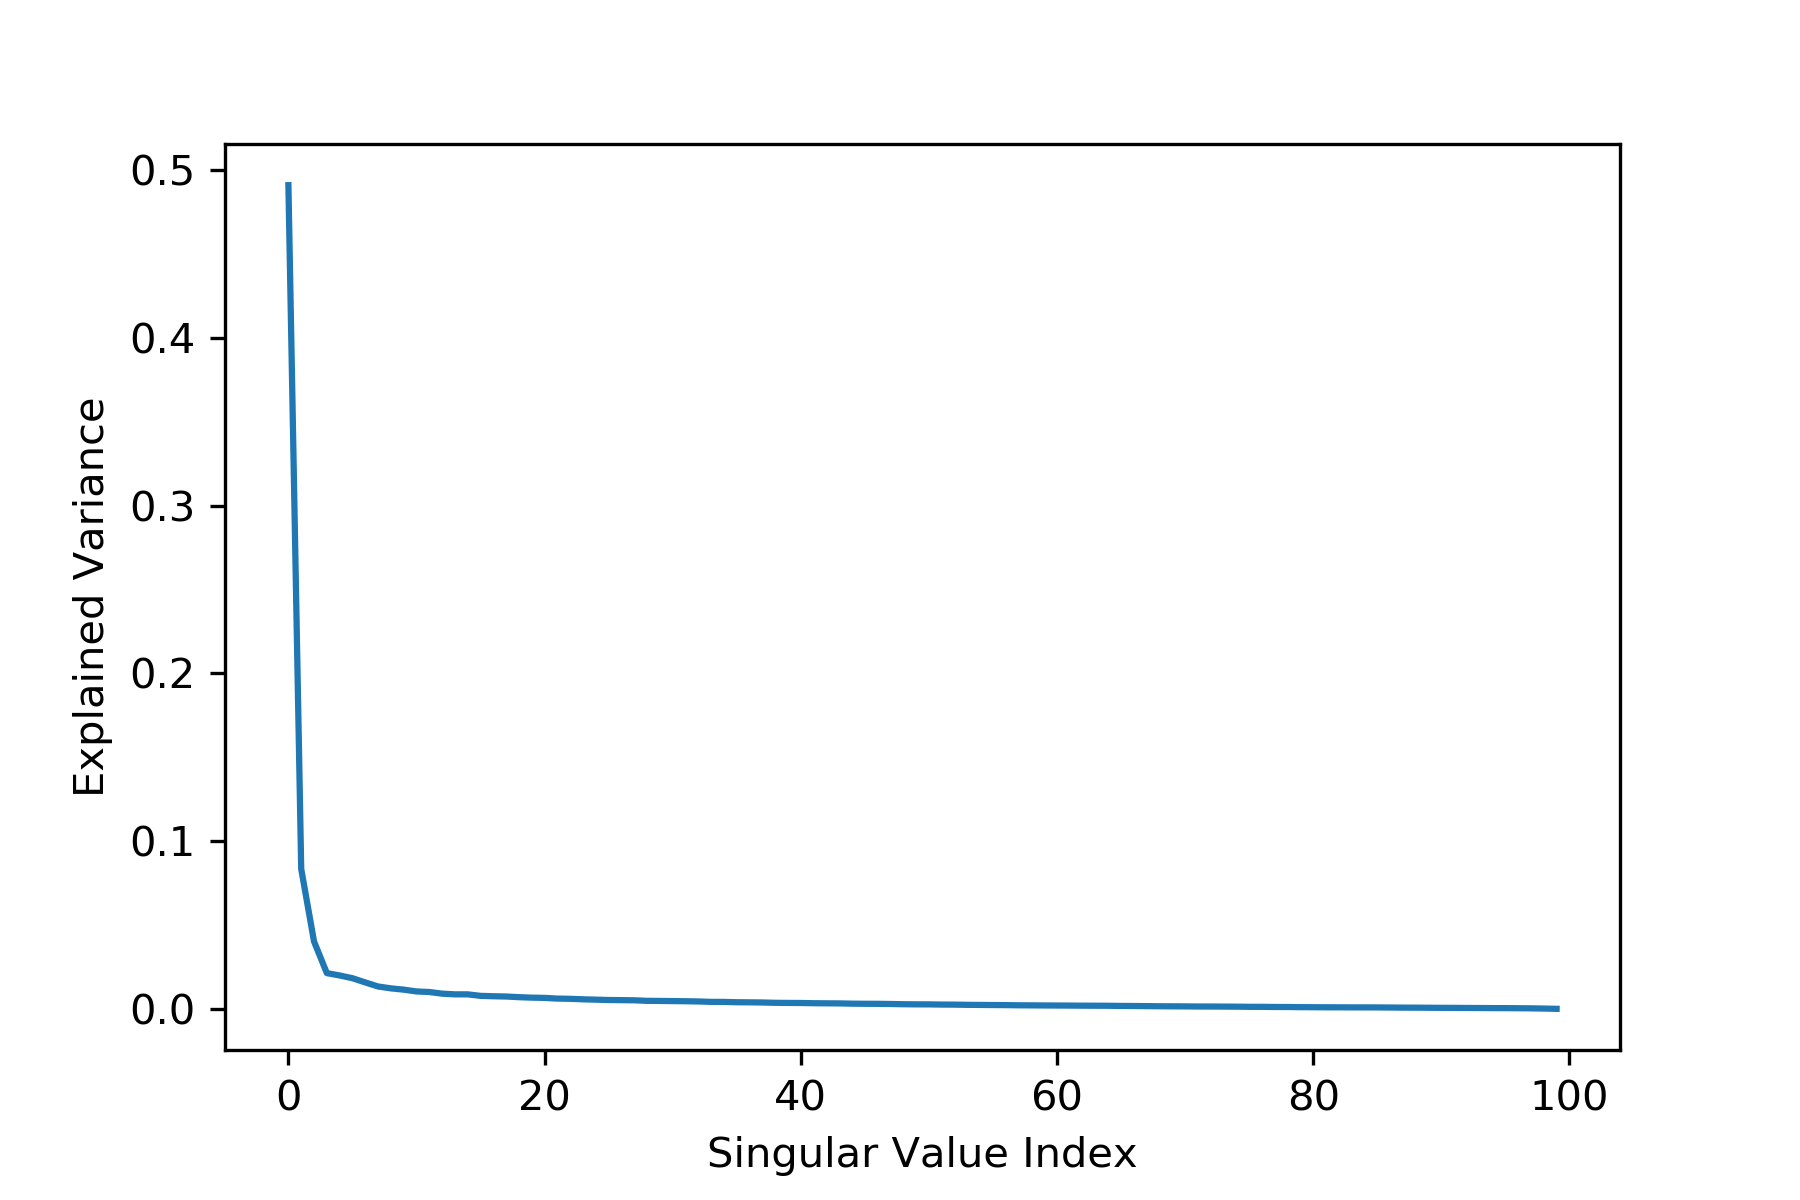
\includegraphics[width=0.5\textwidth]{figs/explained_variance.png}}
\end{figure}

\begin{minted}[breaklines]{python}
fig = plt.figure(figsize = (8,8))
ax = fig.add_subplot(1,1,1)
ax.set_xlabel('Principal Component 1')
ax.set_ylabel('Principal Component 2')
ax.set_title('2-PCA Projection')
for senator in range(100):
    ax.scatter(X[senator,:] @ pca.components_[0,:], X[senator,:] @ pca.components_[1,:], c=affiliations[senator])
\end{minted}
\begin{figure}[H]
    \centerline{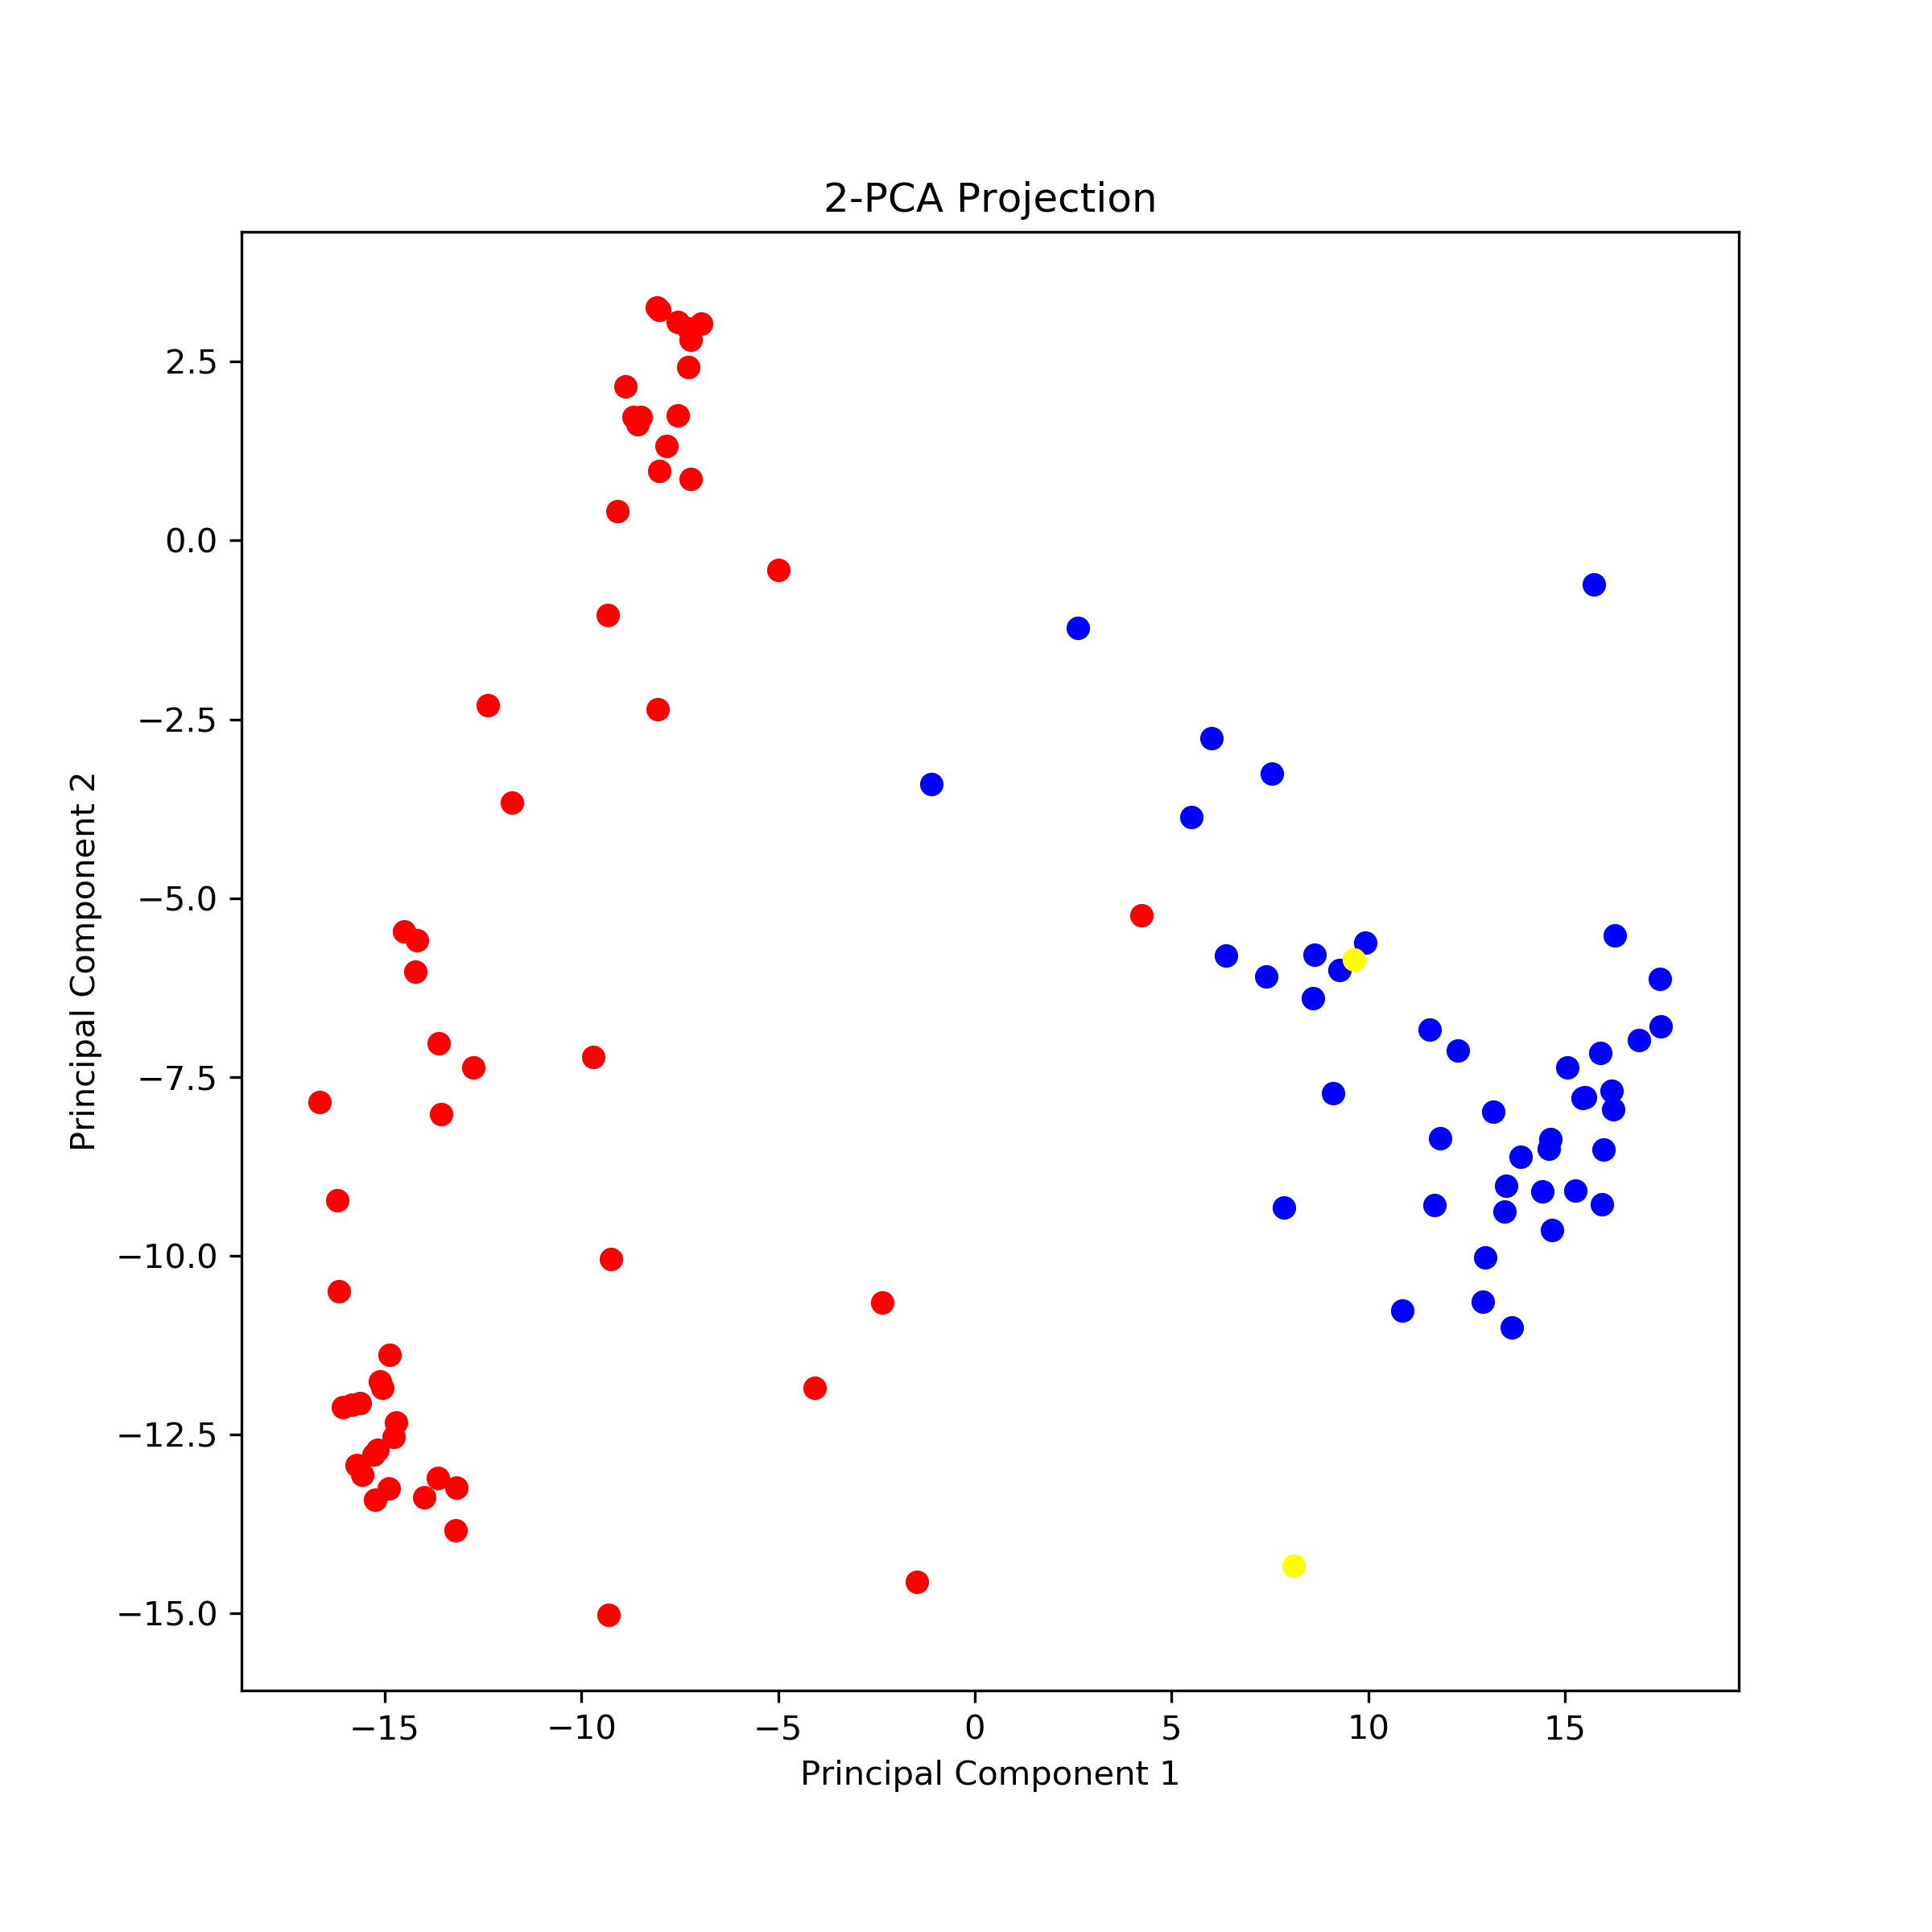
\includegraphics[width=0.5\textwidth]{figs/pca_projection.png}}
\end{figure}

\item
\begin{minted}{python}
np.argmax(pca.components_[0,:])
15
\end{minted}
And it looks like some abortion bill, so makes sense as the most useful bill to split votes along party lines.

\begin{minted}{python}
for senator in range(100):
    senator_scores[senator] = np.abs(X[senator,:] @ pca.components_[0,:])
[(senator_df.columns[i+3], affiliations[i]) for i in np.argsort(senator_scores)[::-1]]
\end{minted}
The 'most extreme':
\begin{minted}{text}
[(' PaulS.Sarbanes(MD)', 'Blue'),
 (" EdwardM.'Ted'Kennedy(MA)", 'Blue'),
 (' BarbaraBoxer(CA)', 'Blue'),
 (' JonKyl(AZ)', 'Red'),
 (' FrankR.Lautenberg(NJ)', 'Blue'),
 (' CarlLevin(MI)', 'Blue'),
 (" JamesM.'Jim'Inhofe(OK)", 'Red'),
\end{minted}
\end{enumerate}
\end{solution}

\newpage
\subsection*{Exercise 4 (Diet Planning)}

We consider a set of $n$ basic foods (such as rice, beans, apples) and a set of $m$ nutrients or components (such as protein, fat, sugar, vitamin C). Food $j$ has a cost given by $c_j$ (say, in dollars per gram), and contains an amount $N_{ij}$ of nutrient $i$ (per gram). (The nutrients are given in some appropriate units, which can depend on the particular nutrient.) A daily diet is represented by an $n$-vector $d$, with $d_i$ the daily intake (in grams) of food i.

\begin{enumerate}
    \item Express the condition that a diet $d$ contains exactly the total nutrient amounts given by the m-vector $n_{des}$, and has a total cost $B$ (the budget) as a set of linear equations in the variables $d_1, ..., d_n$. (The entries of $d$ must be nonnegative, but we ignore this issue here.)

    \item Now suppose we are given $n + 1$ new constraints that requires how different the daily diet $d$ is from some predetermined set diet $s_i \in \mathbb{R}^n$, for $i = 1, ..., n+1$, using the 2-norm as a measure of difference. That is, we have
    $$
    \| d - s_i \|_2 = p_i
    $$
        Express these constraints as a set of $n$ constraints \textbf{linear} in $d$ (\textbf{Correction:} and a \textbf{single} additional constraint that is quadratic in $d$.
\end{enumerate}

\begin{solution}
\begin{enumerate}
    \item We can express the first condition (diet $d$ will lead to consumption of nutrition vector $n_{des}$)
        \begin{align*}
            N d = n_{des}
        \end{align*}
        where $N$ is constructed of $N_{i,j}$ values and is (m x n), $d$ is (n x 1), and $n_{des}$ is (m x 1).

        The second condition (diet $d$ has total cost $B$)
        \begin{align*}
            c^T d = B
        \end{align*}
        where $c$ is a vector of $c_j$ cost for each food and $B$ is the budget.

    \item \textbf{TODO TODO TODO}
\end{enumerate}
\end{solution}

\newpage
\subsection*{Exercise 5 (A result related to Gaussian distributions)}

Let $\Sigma \in S^n_{++}$ be a symmetric, positive definite matrix. Show that
$$
\int_{\mathbb{R}^n} e^{-\frac{1}{2}x^T \Sigma^{-1} x} dx
= (2 \pi)^{\frac{n}{2}} \sqrt{\text{det} \Sigma}.
$$
\textbf{You may assume known that the result holds true when $n = 1$}. The above shows that the function $p : \mathbb{R}^n \rightarrow \mathbb{R}$ with (non-negative) values
$$
p(x) = \frac{1}{(2\pi)^{n/2} \cdot \sqrt{\text{det} \Sigma}} e^{-\frac{1}{2} x^T \Sigma^{-1} x}
$$
integrates to one over the whole space. In fact, it is the density function of a probability distribution called the multivariate Gaussian (or normal) distribution, with zero mean and covariance matrix $\Sigma$.
$$
\int_{x \in \mathbb{R}^n} f(x)
=
|\text{det} P| \cdot \int_{z \in \mathbb{R}^n} f(Pz) dz.
$$

\begin{solution}
\begin{align*}
    \text{For } n = 1&: \int_{\mathbb{R}} \exp(-\frac{1}{2} x \Sigma^{-1} x) dx = \sqrt{2 \pi} \sqrt{\Sigma} \text{ given} \\
    \text{Using spectral thm } \Sigma &= U^T \Lambda U \rightarrow \Lambda = U \Sigma U^T \\
    \text{Applying inverse } \Sigma^{-1} &= U \Lambda^{-1} U^{-1} \rightarrow \Lambda^{-1} = U^{-1} \Sigma^{-1} U \\
    \text{Note } U^T &= U^{-1} \text{ due to orthogonality} \\
    \text{Let } y &= U^T x \\
    \text{Rewrite integral } &\int_{\mathbb{R}^n} \exp(-\frac{1}{2} y^T \Lambda^{-1} y) dy \\
    &= \int \exp(-\frac{1}{2} \begin{bmatrix} y_0 & \dots & y_n\end{bmatrix} diag(\lambda_0^{-1} \dots \lambda_n^{-1}) \begin{bmatrix} y_0 \\ \vdots \\ y_n \end{bmatrix}) dy \\
    &= \int \exp(-\frac{1}{2} (y_0^2 \lambda_0^{-1} + \dots + y_n^2 \lambda_n^{-1}) dy \\
    &= \prod_i^{n} \int \exp(-\frac{1}{2} y_i^2 \lambda_i^{-1}) dy \\
    &= \prod_i \sqrt{2 \pi} \sqrt{\lambda_i} \\
    &= (\sqrt{2 \pi})^n \sqrt{\lambda_0 \dots \lambda_n} \\
    &= (2 \pi)^{\frac{n}{2}} \sqrt{\det \Sigma}
\end{align*}

\end{solution}

\newpage
\subsection*{Exercise 6 (Analysis of calendar days)}

Consider a matrix made up of numerical representations of a range ${\cal T}$ of calendar days. For example, the matrix below represents the range ${\cal T}$ starting on November 1, 2013 and ending on November 3, 2013:
\[
X = \left(\begin{array}{ccc}
2013 &         11       &     1       \\
        2013      &     11        &    2     \\
        2013      &     11     &       3     \end{array} \right)
\]
\begin{enumerate}
    \item Form a matrix $X$ for the date range ${\cal T}$ starting on November 1, 2003 and ending on October 31, 2013.
    \item Find an SVD of the matrix, and print out the right singular vectors and corresponding singular values.
    \item What is the exact rank of $X$?  Numerically, would you say that the rank of the matrix is ``low''? Comment.
    \item Plot the left singular vectors. Do these vectors exhibit a pattern? How would you interpret that pattern?
    \item Explain the significance of the right singular vector $v$ corresponding to the smallest singular value. How would you approximate such a vector by hand?
    \item How would you expect the condition number (ratio from largest to smallest singular value) to behave as the number of calendar days in ${\cal T}$ increases?
\end{enumerate}

\begin{solution}
\begin{enumerate}
\item
\begin{minted}[breaklines,tabsize=2]{python}
T_start = datetime.datetime.strptime("09-01-2003", "%m-%d-%Y")
T_end = datetime.datetime.strptime("09-01-2013", "%m-%d-%Y")
dates = [T_start + datetime.timedelta(days=x) for x in range(0, (T_end - T_start).days)]

X = np.zeros((len(dates), 3))
for i, date in enumerate(dates):
    X[i,0] = int(date.strftime("%Y"))
    X[i,1] = int(date.strftime("%m"))
    X[i,2] = int(date.strftime("%d"))
print(X)
\end{minted}

\item
\begin{minted}{python}
u, s, vh = np.linalg.svd(X)
print(s)
print(vh)
\end{minted}
\begin{minted}{text}
[121378.12798186    531.91591068    208.51159056]
[[-0.99996404 -0.00324745 -0.00783359]
 [-0.00784938  0.00487826  0.99995729]
 [ 0.0032091  -0.99998283  0.00490358]]
\end{minted}

\item The exact rank is 3. The rank is 'low' relative to the number of dates, but that's because we have a non-square matrix with full column rank.

\item The vectors exhibit a pattern that represents the data in years, days, and months respectively.
\begin{minted}{python}
f, ((ax1, ax2, ax3)) = plt.subplots(1, 3, figsize=(30, 7))
ax1.plot(u[:,0])
ax2.plot(u[:,1])
ax3.plot(u[:,2])
\end{minted}

\begin{figure}[H]
    \centerline{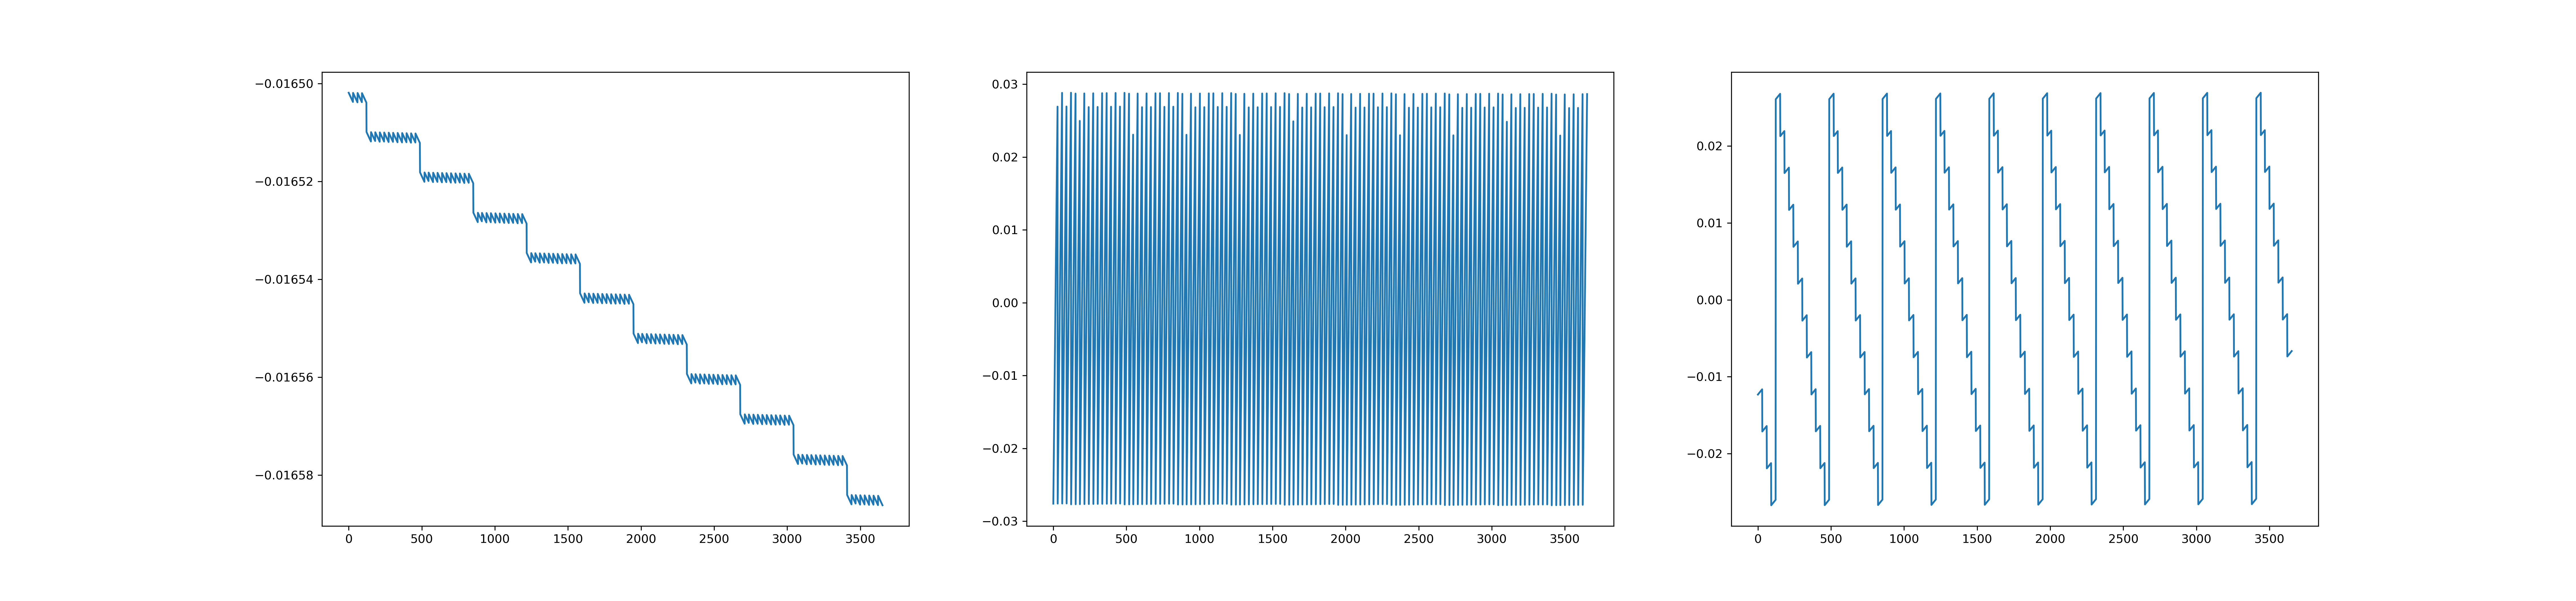
\includegraphics[width=1.2\textwidth]{figs/left_singular_vectors.png}}
\end{figure}

\item The right singular vector corresponding to the smallest singular value is about $\begin{bmatrix} 0 & -1 & 0 \end{bmatrix}^T$. This corresponds to the 'month' column which has the smallest inter-row variance and impact to the norm among each row in $X$. I would estimate $\begin{bmatrix} 0 & -1 & 0\end{bmatrix}^T$ by hand for more than one month worth of entries in $X$.

\item Empirically I see that the condition number increases mildly when I increase the number of entries in $X$. But based on analytic thinking, I wouldn't expect the condition number to increase past a certain point because the right singular vectors approach having $-1$ in only one of their entries (rest zero) and the singular values would just scale together with more entries in $X$.

\end{enumerate}
\end{solution}
\end{document}
